\documentclass{article}
\usepackage[utf8]{inputenc}
\usepackage[italian]{babel}
\usepackage[T1]{fontenc}
\usepackage{hyperref}
\usepackage{graphicx}

\title{Progetto Fine Corso Laboratorio di Reti \newline World Quizzle}
\author{Nicola Dardanis - 579047}
\date{A.A. 2019/2020}

\begin{document}
    \maketitle
    \newpage

    \tableofcontents
    \newpage

    \vspace{2cm} %Add a 2cm space
    \begin{abstract}
        World Quizzle è un gioco online in cui gli utenti registrati al servizio possono creare una propria rete di amicizie e sfidarsi in gare di traduzione di parole. Nel seguito è riportata l'architettura e il funzionamento complessivo del sistema, nonché una descrizione dei packages e delle principali scelte implementative. Sono inoltre fornite le istruzioni per la compilazione e l'esecuzione del codice e le varie opzioni d'avvio.
    \end{abstract}
    \newpage


    \section{Architettura generale del sistema}
    Il sistema nella sua interezza presenta un'architettura generale del tipo client-server con protocollo di comunicazione stateful, necessario data la natura a sessione utente di WQ. L'organizzazione del progetto riflette queste componenti nei due sottomoduli \emph{client} e \emph{server}, inoltre è presente un terzo sottomodulo \emph{commons} che fornisce funzionalità condivise ai due applicativi finali.
    \newline
    L'implementazione è stata guidata dall'\textbf{idea di servizio} intesa come componenente che svolge un certo determinato (unico) compito, così da favorire successive modifiche e sviluppi, e dividere la complessità del sistema in componenti il più possibile autonome e trasparenti una all'altra, che forniscono di fatto servizi, nonché facilitare e rendere efficace la stesura di test units. La struttura dei varii packages rispecchia questa concezione. Segue la descrizione completa e dettagliata delle scelte progettuali e del funzionamento dei varii componenti.

    \section{Client}
    \subsection{Servizi}\label{client-services}
    A livello utente l'interazione con il sistema avviene tramite una CLI fornita dall'applicativo client. A livello applicazione il client è composto di:
    \begin{itemize}
        \item servizio TCP per la normale comunicazione con il server, implementato dal singleton \textbf{TCPHandler}. Utilizza la tecnologia \texttt{java.io} con letture/scritture bloccanti sulla socket, poiché questa modilità ben supporta una interazione mediante CLI.
        \item il servizio di lettura delle notifiche di richiesta di sfida, implementato da \textbf{UDPReader}, anch'esso un singleton come tutti i "servizi" del progetto, che viene attivato su un thread separato ed ascolta in background i pacchetti UDP provenienti dal server, li filtra verificandone la correttezza del contenuto e li pubblica su una BlockingQueue utilizzata per la comunicazione interprocesso con il thread del NotificationCosumer, descritto in seguito (\ref{client_threads}).
        \item il servizio di gestione della cli, fornito nel package cli, in cui il flusso dell'interazione con l'utente è guidato dal \textbf{CliManager} (v.\ref{interact}). In questo package (attraverso il \textbf{NotificationCosumer}) si gestisce anche il display delle notifiche di sfida utilizzando un thread apposito eseguito dall'ingresso all'uscita dell'utente nella "sala d'attesa".
    \end{itemize}

    \subsection{Lifecycle}
    \subsubsection{Start} E' la fase di allocazione delle risorse e settaggio delle configurazioni, in particolare:
    \begin{itemize}
        \item viene instaurata una connessione TCP con il server attraverso la quale avverranno le successive comunicazioni. Un errore in fase di connessione termina il programma, infatti l'impossibilità di connettersi al server compromette l'utilizzo dell'intera applicazione. La connessione è gestita dal TCPHandler (v.\ref{client-services}).
        \item viene istanzato l'UDPReader (v.\ref{client-services}). La porta UDP viene quindi impostata nelle configurazioni di login del client che la comunicherà al server al momento dell'effetiva login. E' stata scelta questa soluzione piuttosto che l'utilizzo di una porta statica per rendere possibile l'esecuzione in locale dell'intero sistema client-server, attivando più processi client contemporaneamente. Anche in questo caso un errore di connessione determina la chiusura del processo.
        \item viene inizializzato il gestore della CLI (\textbf{CliManager} v.s.) e si entra nella fase di interazione (prompt-loop).
    \end{itemize}
    Si noti che in questa fase non viene localizzato il servizio RMI di registrazione di un nuovo utente a WQ in quanto non ritenuto strettamente necessario per lo svolgimento dell'interazione da parte di un utente già registrato al servizio. Per maggiori dettagli si veda \ref{client_RMI} \ref{server_RMI}


    \subsubsection{Interact}\label{interact} In questa fase avviene l'interazione dell'utente con l'applicazione attraverso la CLI, che è modellizzata da una \textbf{macchina a stati finiti} (fig.\ref{fig:client_FSM}) i cui stati sono:
    \begin{itemize}
        \item MAIN: a questo stato è associata la visualizzazione del prompt dei comandi principale che mette a disposizione dell'utente le funzioni di login, logout, show-score, show-friend, show-ranking-list, add-friend, register, ingresso in sala d'attesa (wait-challenge), richiesta di sfida (challenge), exit;
        \item WAIT\_BATTLE: è lo stato in cui si transisce a seguito del comando wait-challenge. Indica quindi che si è nella "sala d'attesa". Entrando in questo stato il CliManager attiva un thread delle notifiche, che sarà disattivato non appena lo si lascia. La CLI mostra la schermata secondaria per la scelta dello sfidante in cui il NotificationCosumer aggiungerà gli sfidanti disponibili per ogni nuovo pacchetto di sfida pubblicato dal servizio UDP.
        \item ONGOING\_BATTLE: indica che c'è una sfida in corso. La CLI mostra il prompt contenente la parola da tradurre;
        \item EXIT: indica la fine dell'interazione dell'utente con la CLI, dopo un messaggio di chiusura si passa alla fase Exit;
        \item ERROR: se si transisce in questo stato non si può transire in nessun altro stato, indica un errore che comporta la chiusura dell'applicazione (si passa alla fase Exit), come un errore di lettura o scrittura sulla socket TCP;
    \end{itemize}

    \begin{figure}[htp]
        \centering
        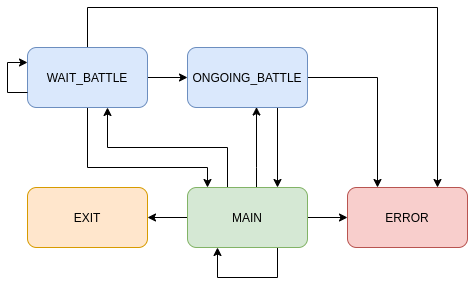
\includegraphics[width=\textwidth]{stati.png}
        \caption{CLI FSM}
        \label{fig:client_FSM}
    \end{figure}

    La CLI è implementata nel \textbf{package cli}, che contiene le definizioni degli stati date sopra, il \textbf{CliManager}\label{CliManager}, un singleton che \textit{si occupa della verifica e delle transizioni di stato} (implementando in maniera naive la funzione di transizione) gestendo dunque anche la creazione e distruzione del thread per le notifiche. La stampa dei prompt e la lettura dell'input sono delegate alle istanze della classe Prompt. Il package contiene a sua volta un sotto-package \textbf{cli.processors} in cui sono definite le classi per processare gli input dell'utente, gli \textbf{InputProcessors}.

    \subparagraph{Prompt} è l'astrazione di una singola interazione dell'utente con la cli, intesa come stampa di un messaggio e richiesta successiva di un input dall'utente legata all'informazione di stato raggiunto al momento della stampa. L'input viene in seguito processato dall'InputProcessor allegato al prompt. \textbf{Tutte le letture da standard input avvengono attraverso il \textit{BufferedReader} istanziato da questa classe} e, dal momento che i prompt vengono eseguiti esclusivamente dal CliManager, si ottiene una gestione consistente e chiara dell'interazione programma/utente, guidata dallo stato interno della CLI.

    \subparagraph{InputProcessor} è l'interfaccia con cui è modelizzata la risposta da parte del programma a un input ricevuto. Di base sono equipaggiati con le due funzioni \emph{validate} e \emph{process} per la validazione e il processing successivo. Sono questi oggetti a gestire individualmente, se necessario, lo scambio dei pacchetti con il server (utilizzando il \textit{TCPHandler}).
    \newline
    \newline
    Si noti come tutta la gestione della CLI avviene per delegazione dei task (il CliManager delega ai Prompt che delegano agli InputProcessors) secondo i principi \emph{composizionale anziché ereditario} e della \emph{separazione degli incarichi}, pur mantenendo \emph{il controllo centralizzato delle risorse e dello stato}, idealmente inspirato dai principali framework grafici come React Redux. Inoltre si è volutamente tenuto slegato il concetto di sessione utente di WQ da quello di interfaccia. Tale legame sarebbe più logico in una GUI, peraltro non difficilmente implementabile come estensione dell'applicativo client fornito, aggiungendo alcuni stati mancanti (come sotto-stati di quelli presenti nella attuale FSM) per modelizzare le varie schermate senza scomporre la logica attuale. Si da quindi la possibilità di registrare nuovi utenti durante una sessione di login, sarà il server a provvedere ai necessari controlli di sessione qualora dei comandi siano inviati dal client prima di un effettivo login. Infine, sempre con lo spirito di lasciare spazio a future estensioni, si osservi come gli InputProcessors siano facilmente riutilizzabili per l'implementazione della GUI, essendo di fatto come delle "callback reificate", secondo un pattern a comandi (\textit{Command Pattern}).

    \subsubsection{Exit} E' il momento precedente alla chiusura dell'applicazione in cui si deallocano tutte le risorse in uso: si chiude la socket TCP nonché gli stream in scrittura e lettura su di essa, si stoppa la lettura dalla socket UDP e si aspetta la terminazione del thread che la gestisce, si stoppa e si aspetta la terminanzione di un eventuale NotificationCosumer attivo e si chiude lo stream per la lettura dallo standard input.

    \subsection{Threads e gestione della comunicazione interprocesso}\label{client_threads}
    Il processo client in fase di inizializzazione attiva un thread per eseguire il servizio di lettura e pubblicazione delle notifiche di sfida provenienti dal server offerto dall'UDPReader. Le interazioni con il server su TCP e la lettura da standard input (interazioni con l'utente) sono invece gestite in maniera bloccante dal processo principale.
    \newline
    Lo schema base dei threads è mostrato in figura \ref{fig:thread_client_1}.
    \begin{figure}[htp]
        \centering
        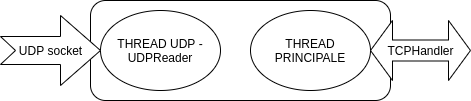
\includegraphics[width=10cm]{threads_client_1.png}
        \caption{Schema base dei threads normalmente attivi}
        \label{fig:thread_client_1}
    \end{figure}

    Un terzo thread viene attivato e disattivato rispettivamente all'ingresso e all'uscita (sia in condizioni normali che di errore) della sala d'attesa per eseguire il NotificationCosumer. Questo comunica con il thread UDPReader attraverso una ArrayBlockingQueue sul quale il servizio di lettura UDP pubblica i pacchetti di notifica e da cui il NotificationCosumer li rimuove (consuma) stampando a schermo il nome dello sfidante associato a un numero progressivo per consertire la scelta all'utente. Si noti la scelta di una ArrayBlockingQueue come mezzo di comunicazione interprocesso, con un numero massimo di 20 elementi, che garantisce l'accesso in mutua esclusione quando necessario. Si noti che è stata scelta una coda limitata per contenere la memoria utilizzata in casi anche di lungo utilizzo dell'applicazione senza l'accesso alla sala d'attesa (nella quale la coda viene invece consumata interamente dal NotificationConsumer), ma un limite di 20 richieste pendenti di sfida verso l'utente è più che ragionevole per una buona esperienza utente. Inoltre si noti che all'arrivo di un nuovo pacchetto di sfida, qualora la coda fosse piena, si procede all'eliminazione del più vecchio pacchetto rimasto in coda e all'inserzione del nuovo secondo la politica FIFO.

    \begin{figure}[htp]
        \centering
        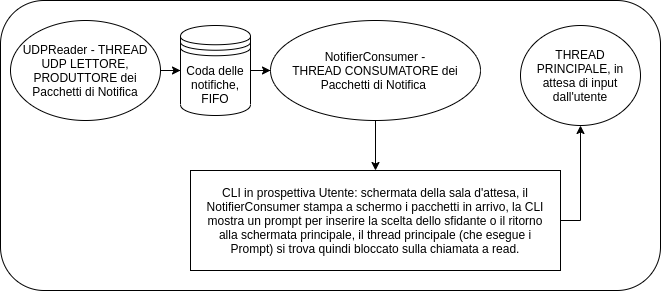
\includegraphics[width=\textwidth]{threads_client_2.png}
        \caption{Schema dei threads attivi in sala d'attesa e loro comunicazione}
        \label{fig:thread_client_2}
    \end{figure}

    \subsection{Utilizzo del servizio di registrazione} \label{client_RMI}
    Il servizio per la registrazione di un nuovo utente al servizio è accessibile durante la fase d'interazione con la CLI attraverso il comando register (v.\ref{client_commands}). Questo utilizza la tecnologia \texttt{RMI} come da linee guida del progetto, ma poiché ritenuto non determinante per l'utilizzo dell'applicazione in un normale use case di un utente già registrato al servizio (molto più comune dello use case in cui un utente non possiede ancora un account e si deve registrare), si è scelta la strategia del "lazy loading", intesa come localizzazione su richiesta dell'oggetto remoto \emph{RegistrationRemoteService} che andrà ad eseguire le nostre richieste. Per maggiori informazioni: \ref{server_RMI}.

    \subsection{Lista dei comandi disponibili}\label{client_commands}
    In riferimento alla FSM descritta per la fase di Interact (v.\ref{interact}) dell'applicazione, l'utente ha a disposizione i seguenti comandi per ognuno degli stati:
    \begin{itemize}
        \item MAIN:
        \begin{itemize}
            \item help: stampa il messaggio di aiuto che mostra i varii comandi disponibili, di cui si fornisce la lista dei parametri e una breve spiegazione.
            \item register <nickname> <password>: registra un nuovo utente a WQ. La password deve contenere almeno 4 caratteri e l'identificativo non può essere scelto tra quelli già registrati;
            \item login <nickname> <password>: effettua il login a WQ, fallisce nel caso in cui l'utente sia già online (ad esempio se si è effettuato l'accesso da un altro terminale);
            \item logout: effettua il logout da WQ, fallisce nel caso in cui l'utente (client) non abbia precedentemente effettuato il login;
            \item add-friend <nickname>: crea la mutua amicizia fra l'utente e nickname, fallisce se non è stato effettuato precedentemente il login;
            \item show-score: mostra il punteggio attuale dell'utente, fallisce se non è stato effettuato precedentemente il login;
            \item show-friend: mostra gli amici dell'utente, fallisce se non è stato effettuato precedentemente il login;
            \item show-ranking-list: mostra la classifica e i relativi punteggi dell'utente e di tutti i suoi amici, fallisce se non è stato effettuato precedentemente il login;
            \item challenge <nickname>: inoltra un pacchetto di sfida all'utente nickname, se nickname accetta si passa alla schermata di sfida, fallisce se non è stato effettuato precedentemente il login. Nota: il server (v.\ref{server}) si occupa dell'inoltro vero e proprio tramite UDP della notifica e della gestione di un eventuale timeout di attesa per fornire il risultato della richiesta all'utente;
            \item wait-challenge: porta l'utente in sala d'attesa, fallisce se non è stato effettuato precedentemente il login;
            \item exit: richiede l'uscita dall'applicazione, a seguito di questo comando si esce dalla fase di Interact.
        \end{itemize}
        \item WAIT\_BATTLE:
        \begin{itemize}
            \item exit (o input vuoto): l'utente esce dalla sala d'attesa e si torna al menù principale;
            \item <n>: un numero tra quelli stampati a schermo del NotifierConsumer, indica l'utente di cui si accetta la richiesta di sfida. Se il numero inserito non è fra quelli visualizzati o il server da un esito negativo si torna al menù principale, se invece va a buon fine si passa alla schermata di sfida;
        \end{itemize}
        \item ONGOING\_BATTLE:
        \begin{itemize}
            \item input vuoto: salta la parola corrente che non verrà conteggiata in maniera autonoma rispetto alle parole correttamente/erroneamente tradotte secondo quanto indicato nel regolamento dal server al momento dell'ingresso in sfida;
            \item sequenza di caratteri, contenenti eventualmente spazi: sono interpretati come la traduzione dell'espressione mostrata che l'utente invia al server;
        \end{itemize}
        \item ERROR, EXIT: nessun comando disponibile.
    \end{itemize}

    \section{Server}\label{server}
    Il server è realizzato con multiplexing dei canali mediante \texttt{java.nio} e multithreading sfruttando il supporto fornito dalle \texttt{CompletableFuture} per l'esecuzione asincrona di task bloccanti (accessi allo Storage, chiamate a servizi esterni) e la gestione delle sfide. Questa scelta è stata preferita rispetto a un server esclusivamente multithreaded per garantire maggior scalabilità e efficienza del sistema, inoltre sfruttando le potenzialità offerte dalle CompletableFuture si è puntato a uno stile più fluido, dichiarativo e composizionale nella scrittura del codice, seguendo la  già citata idea della \textit{composizione}.

    \subsection{Servizi}
    Il codice del server è suddiviso in servizi, rispecchiati nei varii packages come per il client, che forniscono tutte le varie funzionalità in maniera il più possibile trasparente l'uno a l'altro e sono corredati dalle relative test unit, scritte con l'ausilio della libreria esterna \texttt{JUnit 5} (v.\ref{external_libraries}). Segue una descrizione dettagliata di ogni package e relativo servizio.

    \subsubsection{Configurazioni}\label{server_configurations}
    Nel package \emph{configurations} è contenuta la sola classe \textbf{Config}, si tratta di un singleton che rappresenta la configurazione (e i valori di default) delle opzioni del server, resa così accessibile in ogni punto del codice con facilità. Espone un metodo per il parsing dei parametri in input al programma, e i varii getters per ogni campo privato. Per scopi puramente di debug è serializzabile in JSON. Le opzioni di avvio del server sono elencate in tabella \ref{table:server_config_options}, indicante per ognuna la semantica, il tipo atteso del valore e il valore di defaut.

    \begin{table}[ht!]
        \centering
        \begin{tabular}{ |c|p{4cm}|c|p{4cm}| }
         \hline
         \textbf{NAME} & \textbf{INFO} & \textbf{TYPE} & \textbf{DEFAULT} \\
         \hline
         setDebug & abilita la modalità debug (es. stampa di informazione aggiuntive) & boolean & false \\
         \hline
         useTranslationCache & abilita la cache per le traduzioni & boolean & true \\
         \hline
         cacheMaxSize & numero massimo di parole da tenere nella cache delle traduzioni & int & 1000 \\
         \hline
         useISOSourceLang & lingua in cui è scritto il dizionario, in formato ISO 639-1 & string & it \\
         \hline
         useISODestinationLang & lingua delle traduzioni, in formato ISO 639-1 & string & en \\
         \hline
         useStoragePolicy & policy per accesso in scrittura sui file, con valori per la scrittura immediata (IMMEDIATELY) e al logout di un utente (ON\_SESSION\_CLOSE) & enum & ON\_SESSION\_CLOSE \\
         \hline
         useStoragePath & path dalla module working directory per la cartella nella quale lo storage effettua il salvataggio dei files & string & internal \\
         \hline
         useDictionary & path dalla module working dirctory per il file dizionario & string & /src/main/resources/\newline dictionary.txt \\
         \hline
         wordsForChallenge & numero di parole per sfida & int & 10 \\
         \hline
         challengeRequestTimeout & tempo massimo di attesa per richiesta di sfida in ms & int & 5000 \\
         \hline
         challengeTime & tempo totale massimo per sfida in s & int & 50 \\
         \hline
         setWordMalus & punti da sottrarre per risposta sbagliata & int & 1 \\
         \hline
         setWordBonus & punti da aggiungere per risposta corretta & int & 3 \\
         \hline
         setWordSkip & punti da aggiungere per risposta saltata & int & 0 \\
         \hline
         setWinnerExtraPoints & punti da aggiungere al vincitore della sfida & int & 5 \\
         \hline
        \end{tabular}
        \caption{Configurazioni di avvio del server}
        \label{table:server_config_options}
    \end{table}

    \subsubsection{Gestione del dizionario e delle traduzioni}\label{server_translations}
    Il package \emph{translation} realizza il servizio per la creazione di dizionari (con traduzione) da utilizzare durante le sfide. Il codice è thread-safe per abilitare la richiesta di dizionari da parte dei vari threads di sfida in parallelo. Al suo interno è suddiviso in due sotto-servizi:
    \begin{itemize}
        \item \textbf{TranslationService}: data una parola ne fornisce la traduzione. Si assume la configurazione linguistica data dall'oggetto Config (v.\ref{server_configurations}), ma permette anche il cambiamento a runtime, per maggiori dettagli si veda sotto;
        \item \textbf{DictionaryService}: Un singleton che si occupa di caricare in memoria il file del dizionario fornito come risorsa statica del server. Fornisce i metodi per richiedere la traduzione parallelo di una lista di n parole, scelte a caso tra quelle del dizionario, e per richiedere la traduzione in parallelo di una lista di parole fornite dal chiamante.
    \end{itemize}

    Nel package è definita anche una eccezione checked (UnavailableTranslationException) che viene utilizzata per segnalare l'impossibilità da parte del servizio di tradurre una data parola.

    \paragraph{Organizzazione interna del servizio di traduzione} \emph{TranslationService} è l'interfaccia del servizio di traduzione, offre i metodi per le configurazioni delle lingue di ingresso/uscita, per la traduzione di una data parola, ed il metodo setNext per la realizzazione del pattern \textbf{Chain Of Responsability}, secondo il quale la traduzione può avvenire a più livelli, se un livello non conosce la traduzione o non riesce a ottenerla, passa la parola da tradurre al livello immediatamente successivo; se nessuno dei livelli forniti riesce a tradurre la parola, viene lanciata l'eccezione \emph{UnavailableTranslationException}. Questa organizzazione rende la gestione delle traduzioni facile ed espandibile, mantenendo chiarezza e pulizia nel codice. Inoltre questa "delegazione a livelli" si presta bene alla risoluzione di un problema nel quale, come nella realizzazione presentata, è utile un servizio di cache, anche a più livelli, o nel quale si vogliano gestire in modo preferenziale, ma non esclusivo, varie fonti di traduzione (ad esempio: cache, traduzioni su disco, db o servizi di terze parti).

    \subparagraph{Cache} \textit{TranslationsPool} è la classe con cui si realizza la cache per ottimizare le performance, diminuendo il numero di chiamate al servizio esterno \emph{MyMemory}. Di base utilizza una \textbf{ConcurrentHashMap} per assicurare l'accesso concorrente alla risorsa, dove vengono memorizzate le parole richieste al servizio con la relativa lista delle traduzioni. Può essere disattivata con una opzione di avvio (tab.\ref{table:server_config_options}) e ha una dimensione limite anch'essa impostabile. I valori della mappa vengono rappresentati attraverso una sottoclasse privata (poiché non di utilità al di fuori di questa classe), assegnando a ognuno di essi il timestamp di ultima lettura così da realizzare una politica di aggiornamento degli elementi "\textbf{on touch}". Inoltre ad ogni lettura di una entry si aggiorna un contatore che indica le volte in cui la risorsa è acceduta. Il primo elemento a essere rimosso sarà quello acceduto meno recentemente (\textit{politica LRU}) di tutti e a parità di timestamp quello meno acceduto storicamente. La mappa nella sua interezza invece ritiene tutti gli elementi e procede al rimpiazzo solo su necessità, in mancanza di slot liberi. Da notare anche la gestione di un eventuale cambio di lingua a runtime (disponibile nel servizio anche se non utilizzato nella attuale realizzazione del progetto) in cui la cache viene invalidata così da assicurare la congruenza fra impostazioni di lingua e traduzioni.

    \subparagraph{MyMemoryAPI} Se la cache non contiene la traduzione per la parola richiesta il servizio di traduzione chiama il livello successivo, nell'implementazione corrente offerto dalla classe MyMemoryAPI, che realizza la chiamata all'API di MyMemory dalla quale si legge un JSON (letto mediante le funzionalità di data-bindings della libreria Jackson in un oggetto che rispecchia la struttura della response, ignorando i campi non utilizzati) contenente le traduzioni che vengono raccolte in una lista e ritornate al chiamante.

    \subparagraph{Ottimizzazione e parallelismo} \emph{DictionaryService} provvede, sfruttando la composizionalità delle CompletableFuture, a eseguire in parallelo le chiamate al TranslationService, così da ridurre drasticamente il tempo d'attesa nella ricezione delle risposte introdotto dalla chiamata eventuale a MyMemory. Si osservi come il parallelismo è gestito sia a livello interno del servizio, sia a livello esterno, a causa di chiamate contemporanee al DictionaryService.


%   \begin{figure}[htp]
%        \centering
%        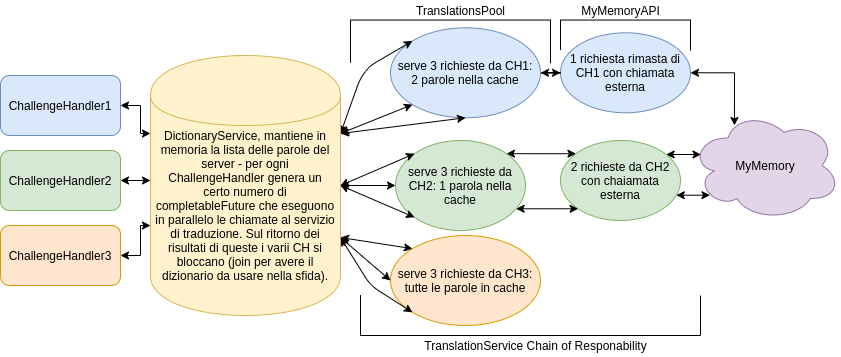
\includegraphics[width=\textwidth]{dictionary.png}
%        \caption{Chiamate parallele al DictionaryService e parellizzazione per ogni CH sulle singole parole nelle chiamate al TranslationService}
%        \label{fig:dictionary_threads}
%    \end{figure}

    \subsubsection{Storage}\label{server_storage}
    Come da specifiche di progetto, il salvataggio delle informazioni degli utenti avviene in formato JSON. Si è scelto però di dividere su due files le informazioni in base a una scala di importanza, in un primo file \emph{registration.json} si salvano le informazioni di registrazione, nome e password dell'utente, nel secondo file \emph{online-info.json} quelle riguardanti l'attività dell'utente, ovvero il suo punteggio attuale e la sua lista di amici. Entrambi i file si trovano all'interno della directory \emph{\$\{module-working-directory\}/internal/} che viene creata all'avvio se non presente.
    \newline
    \paragraph{UserStorage} è il singleton che offre il servizio di gestione del "db utenti". E' contenuto nel package \textbf{storage}, così come l'implementazione del servizio RMI (v. \ref{server_RMI}). UserStorage inoltre mantiene in una \textbf{ConcurrentHashMap} i soli utenti online in memoria (di questi si caricano nella mappa solo le informazioni contenute in \textit{online.json} che sono le uniche che possono variare e a cui si fa riferimento dopo il login), rendendo così trasparente al resto della applicazione l'effettiva presenza di un storage fisico, le informazioni di un utente saranno, infatti, sempre messe a disposizione e accessibili solo attraverso questo servizio, garantendo consistenza dei dati e manutenibilità del sistema. La scelta di mantenere in memoria solo le informazioni degli utenti online anziché tutti quelli registrati a WQ assicura maggiore efficienza e scalabilità. Inoltre si è preferita la hashmap per assicurare un accesso a basso costo, rispetto a una struttura a grafo, che sarebbe inoltre stata in conflitto con il modello di caricamento "on-demand" degli utenti, costringendo il caricamento a catena di tutta la rete di amicizie di ogni singolo utente a partire dal primo necessario. In generale se immaginiamo il grafo degli utenti di WQ come un insieme di n grafi (n>0) non connessi, per poter accedere all'utente i del grafo k avremmo dovuto caricare in memoria l'intero grafo k e non solo l'utente i, con conseguente perdita d'efficienza in termini di tempo e spazio. Ancora, la scelta della mappa è più in linea anche con la rappresentazione delle informazioni dei singoli utenti, in cui troviamo la lista degli amici (v.\ref{server_user}).

    La differenziazione dei dati nei due file si rispecchia anche nelle politiche e metodologie di aggiornamento: il primo infatti è aggiornato non appena si riceve un comando di registrazione corretto, mediante un apposito task che per ottimizzare la scrittura su file appende il nuovo oggetto registration-utente (v.\ref{server_user}), così da non dover scorrere e copiare l'intero file, il secondo invece necessita di aggiungere nuovi utenti (stesso meccanismo descritto sopra), ma anche di aggiornarli: l'aggiornamento è attuato mediante scorrimento e copia dell'intero file (v.\ref{server_ioTasks}). Inoltre sul secondo file è possibile impostare, mediante una opzione di configurazione, una delle due politiche di accesso descritte dall'enum \textbf{Policy} (tab. \ref{table:server_config_options}):
    \begin{itemize}
        \item IMMEDIATELY: politica "write on change", i file su disco vengono aggiornati non appena si aggiorna lo stato di un utente.
        \item ON\_SESSION\_CLOSE: in questà modalità si trattano in modo diverso gli utenti online (soggetti a modifiche più di frequente) rispetto agli altri, per i quali continua a valere la precedente politica. Per ottimizzare gli accessi al disco si aggiornano i dati di un utente online su file solo al momento del suo logout. Notiamo che qualora si dovesse verificare un imprevisto down del server, si andrebbero a perdere solo informazioni non sensibili, poiché i dati di registrazione vengono sempre scritti solo al momento della registrazione, nel file registration.json.
    \end{itemize}

    Da notare che l'utilizzo di UserStorage è completamente thread-safe ad accessi concorrenti, sia per quanto riguardo l'accesso agli utenti già caricati da disco (grazie alla concurrentHashMap come menzionato sopra) sia per le operazioni su files, protette attraverso una \textbf{ReadWriteLock} così da permettere l'accesso concorrente in sola lettura e in mutua esclusione in scrittura.

    \paragraph{Models}\label{server_user} è il sotto-package di storage in cui sono contenute le classi per la modelizzazione dei dati nel db. In concreto abbiamo una classe \textbf{User} con la quale si rappresenta un utente di WQ, con i suoi dati di login (nome e password), la lista dei suoi amici e il suo attuale punteggio. User fornisce anche altre funzioni utili per la sincronizzazione dell'utente con lo storage fisico, come il meccanismo di tracciamento automatico di eventuali modifiche avvenute per controllare una scrittura ottimizzata. La classe è serializzabile in JSON secondo le \textit{viste} fornite nell'interfaccia \textbf{UserViews}, che sono due, \textit{Registration} e \textit{Online}, e permettono di trattare un utente esattamente secondo il formato atteso nei relativi files. Si sono volute qua sfruttare le annotazioni fornite dalla libreria \texttt{Jackson} per creare in un certo qual modo il concetto di vista che si trova spesso nelle basi di dati relazionali o ad esempio anche nei buffer o stream di dati.

    \paragraph{IoTasks}\label{server_ioTasks} contiene le funzionalità per operare le letture e le scritture sui files. In JSONMapper è present una unica istanza di \texttt{ObjectMapper} (come da best-practice di utilizzo della libreria Jackson) usata per effettuare la scrittura e la lettura dei files dello storage, configurata per fare uso del meccanismo delle Views (v. \ref{server_user}). Sono inoltre fornite funzioni di utilità per la ricerca e l'update degli utenti nei files. \textbf{JSONUserAppender} è invece un Runnable contenente il codice per la creazione di un nuovo utente nel db in modo ottimizzato, senza scorrere tutto il file, e viene utilizatto da UserStorage per aggiungere un nuovo utente parallelamente in fondo a entrambi i files.

    \subsubsection{Registrazione utenti}\label{server_RMI} RegistrationRegistry è il singleton che implementa l'interfaccia \textbf{RegistrationRemoteService} esposta nel modulo \textit{commons}, costituendo di fatto il servizio di registrazione su \texttt{RMI} come richiesto nelle linee guida. Effettua chiamate allo UserStorage per verificare la presenza del nome utente nel sistema (un nuovo utente può registrarsi solo con un nome utente non già presente in WQ) e la scrittura effettiva delle informazioni di login su file. Da notare il fatto che i metodi sono \texttt{synchronized} per assicurare che il controllo sull'unicità del nome utente venga svolto correttamente; RMI infatti non gerantisce che chiamate, anche se thread-safe a livello di JVM del singolo client, siano sincronizzate dall'oggetto remoto: in altre parole non c'è sincronizzazione fra clients diversi. Si potrebbe allora verificare che due clients vogliano registrare contemporaneamente lo stesso identificativo utente, portando possibilmente a una doppia registrazione, causa elusione del controllo di unicità dovuto a una corsa critica fra la richiesta di controllo della seconda registrazione e l'effettiva scrittura della prima.

    \subsubsection{Notifiche di sfida}\label{server_challenge_notification}
    Il \textbf{NotifierService} è il singleton che implementa il servizio per la gestione delle notifiche di sfida per la fase di SETUP (v.\ref{server_challenge_phases}) ed è contenuto nel package \textbf{challenge}. Al momento della istanziazione, si occupa anche di aprire la connessione UDP alla porta 6001 (configurabile in \textit{commons.Config}) per l'invio dei pacchetti di notifica ai clients.
    Mantiene al suo interno due mappe concorrenti, una dai nomi utenti nel loro oggetto di stato della connessione (v.\ref{server_lifecycle}), utilizzata in primo luogo per recuparare la porta UDP dell'utente a cui spedire la notifica di sfida, e l'altra contenente le richieste pendenti di sfida, indirizzata per nome del richiedente. Notiamo che una mappa delle connessioni attive per nome utente, escluse le funzionalità di sfida, sarebbe stata ridondante, ed è per questo che è proprio il NotifierService a mantenerla, unico vero utilizzatore di questa informazione oltre al thread di sfida (v. \ref{server_challenge_phases}), che la sfrutta per registrare i socketChannel dei clients sui selettori secondario in entrata e, in uscita, sul primario.
    \newline Le notifiche di sfida dal server ai clients sono gli unici pacchetti del sistema che viaggiano su UDP, le risposte di accettazione di sfida vengono invece gestite come normali comandi su connessione TCP, così da non dover gestire l'eventuale perdita di pacchetti e/o assicurare che i clients non rimangano mai bloccati perennemente in attesa di una sfida accettata ma, per problemi di rete, non notificata dai clients al server (v. \ref{server_challenge_phases}).

    \subparagraph{Implementazione delle notifiche}
    La realizzazione si basa sulla possibilità di completare manualmente una \texttt{CompletableFuture} attraverso il metodo \texttt{complete} fornito dall'API. Una notifica è infatti una CompletableFuture contenente un timer (configurabile, v.\ref{server_configurations}), implementato con una chiamata a \texttt{Thread.sleep}, allo scadere del quale viene restituito il pacchetto di default (contenente il messaggio di errore nel setup della sfida) da mandare al richiedente e/o al destinatario della richiesta di sfida, a seconda dello stato raggiunto da quest'ultimo. Se invece il destinatario della richiesta, riceve la notifica e accetta la sfida prima dello scadere del timer, la CompletableFuture salvata nella mappa delle richieste pendenti viene completata manualmente con un pacchetto di corretto setup, che verrà inviato a entrambi i giocatori. Nello specifico, il richiedente della sfida sarà bloccato in attesa di risposta, ovvero in attesa del completamento del timer di notifica, nel frattempo il destinatario invierà  l'accettazione che provocherà un completamento del timer di notifica, per cui entrambi gli utenti riceveranno il pacchetto di corretto setup della sfida.

    \subsection{Lifecycle}\label{server_lifecycle} L'applicativo server attraversa una prima Setup phase, in cui legge le opzioni da riga di comando (\ref{server_configurations}), istanza il servizio di traduzione (\ref{server_translations}), componendo cache + gestione dell'api esterna, istanza lo storage utenti con le configurazioni di percorso dei file (\ref{server_storage}), crea e attiva il processo del registry RMI sulla porta 2020 e esporta il RegistrationRegistry (\ref{server_RMI}), crea il selettore principale, la coda per le registrazioni asincrone degli interessi di lettura e scrittura delle chiavi dei clients (\textbf{connection.AsyncRegistrations}), e apre la socket per l'accettazione dei client alla porta 6000 (configurabile in \textit{commons.Config}), registrandola sul selettore. Infine istanza il NotifierService (\ref{server_challenge_notification}). Il fallimento di una qualsiasi di queste operazioni determina la chiusura dell'applicativo server.
    \newline In seguito viene avviato il classico loop centrale (Main phase) in cui si accettano nuovi clients: si crea un socketChannel registrandolo sul selettore in sola lettura, a cui si allega un'oggetto \textbf{connection.State} per mantenere lo stato della nuova connessione (come nome del client dopo il login, pacchetti da scrivere, bytes ricevuti e non ancora interpretati, porta udp per le notifiche). Il selettore principale si blocca (indefinitivamente) in attesa che un canale sia disponibile per una delle operazioni richieste, in particolare (inizialmente) si aspetta di leggere un comando dai clients. Quando a seguito di una o più operazioni di lettura si compone un pacchetto, questo viene interpretato e, a seconda dell'\texttt{operationCode} in esso contenuto, si eseguono le azioni corrispondenti, con l'accortezza di svolgere tutte le operazioni bloccanti in asincrono. Alcune delle operazioni non sono riconosciute nel thread principale, che registra nuovamente il client in lettura ignorandole (v. \ref{protocol_operations}). Gli errori che si verificano nello svolgimento delle varie operazioni sono tutti gestiti su varii livelli e possono comportare al più la chiusura della connessione verso il client che ne ha fatto richiesta.

    \subsection{Sfide}
    Le gare di traduzione sono al centro dell'interazione dell'utente in WQ. L'implementazione di una sessione di sfida richiede l'utilizzo di varii servizi, quali in prima istanza, il servizio per la creazione di un dizionario (v. \ref{server_translations}), quello quindi di traduzione, del servizio di notifica (v. \ref{server_challenge_notification}), nonché dello storage utenti (v. \ref{server_user}). E' possibile configurare il numero di parole, punti bonus, malus e tempo limite per le sfide, nonché le lingue e il percorso del file di dizionario da utilizzare per la creazione delle liste di parole che il sistema chiede agli utenti di tradurre (v. \ref{server_configurations}).

    \subsubsection{Fasi}\label{server_challenge_phases} Una sfida fra due utenti attraversa tre macro-fasi:
    \begin{itemize}
        \item SETUP: il server riceve dal richiedente (client1) un pacchetto di richiesta di sfida contenente il nome di un amico (client2), controlla che quest'ultimo sia online e che sussista effettivamente una relazione di amicizia fra i due. In tal caso, tramite il NotifierService, invia una richiesta di notifica (su UDP) a client2. Si attende quindi una risposta affermativa da client2 (v. \ref{client_commands}). Se questa viene ricevuta prima del timeout della notifica (\ref{server_configurations}) si istanza un thread di sfida (vedi fase successiva). Si setta in scrittura il pacchetto di corretto setup ottenuto dal NotifierService per entrambi i clients e si annota nell'oggetto che rappresenta lo stato delle connessioni degli utenti interessati l'impossibilità da parte del selettore principale di leggere i socketChannel. Questo pacchetto di conferma (contenente le istruzioni di gioco) verrà quindi scritto quando il selettore primario permetterà la scrittura ai clients, la risposta verrà invece letta sbloccando il selettore secondario attivato dal thread di sfida, bloccato in attesa che i due canali risultino leggibili.
        \item CHALLENGE: gestita interamente dal Runnable \textbf{ChallengeHandler}, creato e mandato in esecuzione nella fase precedente, contiene la creazione del dizionario, con eventuale gestione e uscita in caso di fallimento (cancellazione delle chiavi dal selettore secondario e invio tramite selettore primario del pacchetto di errore), la gestione dei socketChannel tramite loop su \textit{selettore secondario con timeout}, impostato su un secondo, (necessario proprio per controllare lo scorrere del tempo durante lo svolgimento della prova e/o controllare eventuali situazioni di errore senza rimanere bloccati) con invio e ricezione dei varii pacchetti contenenti le parole da tradurre e le traduzioni,
        il conteggio dei punti e il timeout di sfida (\ref{server_configurations}), alla cui scadenza la sfida si considera conclusa (con successo, si procede a designare il vincitore) anche se uno o entrambi i giocatori non hanno ancora finito di tradurre tutte le parole.
        \item EXIT\_CHALLENGE: si procede alla chiusura del thread di sfida e al reinserimento in lettura/scrittura dei canali sul selettore principale. Se si verifica un errore in una delle fasi precedenti si salta subito a questa fase, si cancellano le chiavi secondarie e si ri-registra l'interesse in scrittura per entrambi i clients sul selettore primario settando come prossimo pacchetto in scrittura un pacchetto di chiusura fallimentare della sfida. Se invece la sfida si conclude correttamente vengono confrontano i punteggi ottenuti, si stabilisce il vincitore aumentando il suo punteggio dei punti vincita, si procede quindi a chiamare lo UserStorage per l'aggiornamento dei punteggi dei due giocatori e infine si compone il messaggio di fine partita che sarà il prossimo pacchetto da scrivere e, come nel caso precedente si procede con la cancellazione delle chiavi secondarie e il reinserimento sul selettore principali.
    \end{itemize}



    \section{Protocollo di interazione}
    \label{protocol}
    \subparagraph{Protocollo di rete TCP/UDP} Il modulo \textit{commons} fornisce le classi di utilità per la gestione dei \textbf{pacchetti di rete} in WQ, nel package \textbf{protocol}, al fine di fornire a entrambi gli applicativi le funzionalità di base per costruire i pacchetti e serializzarli e deserializzarli nel formato corretto. Il protocollo è stato ideato per una tipica interazione del tipo client-server.
    \subparagraph{Protocollo RMI} Per quanto riguarda invece il protocollo di comunicazione per la registrazione di un nuovo utente su RMI (package \textbf{RMIRegistrationService}), l'invocazione del metodo sull'oggetto remoto di tipo RegistrationRemoteService restituisce un codice di stato di tipo \textbf{RegistrationResponseStatusCode}:
    \begin{itemize}
        \item OK: La registrazione è avvenuta con successo;
        \item INVALID\_NICK\_ERROR: Il nome utene una stringa vuota (o null);
        \item NICK\_ALREADY\_REGISTERED\_ERROR: Il nome utente è già presente in WQ, non sono ammessi dupliati;
        \item INVALID\_PASSWORD\_ERROR: La password è invalida. Una password valida deve contenenere almeno 4 caratteri;
        \item INTERNAL\_ERROR: Si è verificato un errore inatteso.
    \end{itemize}

    \subsection{Formato dei pacchetti di rete}\label{protocol_network}
    Un pacchetto di WQ che viaggia in rete è un oggetto della classe \textbf{WQPacket}, costituito da un \textbf{header} e un \textbf{corpo}. L'header è un solo campo di tipo \texttt{int}, occupa 4 bytes, e contiene la lunghezza dell'intero pacchetto (header + corpo).
    Il corpo è invece un oggetto della classe \textbf{PacketPojo}, contenuto nel sotto-package \textbf{json}, serializzato in JSON. Per essere considerato ben formato il formato deve sempre contenere un codice operazione, per facilitare l'interpretazione del pacchetto e dei suoi campi al ricevente. I pacchetti di risposta contengono anche un codice di risposta, che indica il successo o il fallimento della richiesta. Si veda la tab. \ref{table:commons_packets} per una lista completa dei campi attualmente disponibili.
    \newline La decisione di trattare un pacchetto sotto forma di un oggetto che fornisce un meta-campo e ne incapsula un altro che contiene invece il codice operazione (e risposta) con eventuali paramentri annessi è stata preferita ad altre soluzioni (pacchetto senza header con lunghezze prefissate dei campi, pacchetto contenente nell'header anche il codice operazione, etc.) per ottenere una buona flessibilità, manuteibilità e modificabilità (estensibilità) del protocollo, ed è stata ispirata dall'incapsulamento, idea chiave dei protocolli stratificati. In particolare si volevano evitare codifiche ad-hoc che avrebbero potuto generare confusione e/o rigidità. La presenza della lunghezza nell'header era invece necessaria per una gestione sicura e più efficiente della lettura dei pacchetti mediante \texttt{java.nio} rispetto ad esempio all'uso di caratteri terminatori di pacchetto.
    \newline Si noti che la serializzazione in JSON del pacchetto include solo i campi popolati dell'oggetto PacketPojo, come configurato in \textit{commons.protocol.json.JSOMapper}, motivo per cui non vengono usati tipi primitivi per i campi (tab.\ref{table:commons_packets}), per ridurre i bytes prodotti per il corpo del pacchetto.

     \begin{table}[h!]
        \centering
        \begin{tabular}{ |c|c|p{4cm}|c| }
         \hline
         \textbf{NAME} & \textbf{JSON\_KEY} & \textbf{INFO} & \textbf{TYPE} \\
         \hline
         operationCode & op & operazione richiesta o alla quale si sta rispondendo & OperationCode \\
         \hline
         responseCode & rc & esito dell'operazione & ResponseCode  \\
         \hline
         timestamp & ts & il timestamp di creazione del pacchetto & Long \\
         \hline
         ttl & ttl & time to live, tempo di vita del pacchetto, in secondi  & Integer \\
         \hline
         nickName & name & nome dell'utente, solitamente di chi richiede l'operazione & String \\
         \hline
         password & passw & password dell'utente & String \\
         \hline
         UDPPort & port & porta UDP dell'utente & Integer \\
         \hline
         friend & f & nome di un secondo utente coinvolto nell'operazione richiesta & String \\
         \hline
         word & w & parola da tradurre & String \\
         \hline
         translation & t & traduzione della parola contenuta nel campo word & String \\
         \hline
         message & info & messaggio informativo (spesso usato in caso di errore) & String \\
         \hline
         rankingList & rank & utente e amici con relativi punteggi & List<RankingListItem> \\
         \hline
         friends & fl & lista degli amici di un utente & List<String> \\
         \hline
         scores & s & punteggio di un utente & Integer \\
         \hline
        \end{tabular}
        \caption{Campi di PacketPojo e loro uso tipico}
        \label{table:commons_packets}
    \end{table}

    \subsection{Operazioni}\label{protocol_operations}
    Le operazioni, rappresentate dal'enum \textbf{OperationCode}, sono divise in due gruppi, quelle principali, riconosciute quando lette nel loop del processo principale del server, e quelle invece per la gestione della sfida (riflettendone le fasi v.\ref{server_challenge_phases}), interpretate durante una gara di traduzione e quindi riconosciute nel loop del selettore secondario di sfida (v.\ref{server_lifecycle}):
    \begin{itemize}
        \item Operazioni primarie (selettore primario):
            \begin{itemize}
                \item LOGIN
                \item LOGOUT
                \item ADD\_FRIEND
                \item GET\_FRIENDS
                \item REQUEST\_CHALLENGE
                \item GET\_SCORE
                \item GET\_RANKING
                \item FORWARD\_CHALLENGE
            \end{itemize}
        \item Operazioni secondarie (selettore di sfida):
            \begin{itemize}
                \item SETUP\_CHALLENGE
                \item ASK\_WORD
                \item STOP\_CHALLENGE
            \end{itemize}
    \end{itemize}


    \section{Librerie esterne}\label{external_libraries}
    Per lo svolgimento del progetto sono state utilizzate le seguenti librerie esterne:
    \begin{itemize}
        \item \texttt{Jackson}: per la serializzazione e deserializzazione in JSON del payload dei pacchetti (\ref{protocol}) e degli utenti nello storage \ref{server_storage}. E' stata preferita questa libreria per la ricca API che fornisce, contenente sia le potenti funzionalità di data-binding tramite reflection sia gli oggetti per gestire in maniera puntuale ottimizzata l'albero sintattico del JSON. Nella scrittura dei file nello storage ad esempio è stato utilizzato un approccio che combina queste due caratteristiche per fornire uno scorrimento veloce dei file evitando la creazione di un gran quantitativo inutile di oggetti User (v. \ref{server_user});
        \item \texttt{JUnit5}: per lo sviluppo delle unit tests, con supporto per l'esecuzione parallela.
    \end{itemize}

    \section{Istruzione per l'esecuzione del codice}

    \subsection{Requisiti minimi}
    Per compilare ed eseguire il progetto è necessario installare Java 8 (o superiori) e lo strumento di build management Maven 3 (o superiori).

    \subsection{Build e Test}
    Per buildare il progetto occorre aprire il terminale, spostarsi nella directory principale del progetto contenente il file \textbf{pom.xml} che descrive l'\emph{artifactId} \textbf{world-quizzle} e lanciare il comando \emph{mvn install}.
    Maven scaricherà in automatico le dipendenze esterne (richiesta la connessione a internet) e creerà i jar dei varii moduli (commons, client e server).
    \paragraph{N.B.} Seguendo la procedura descritta si avviano pure i tests, per disabilitarli aggiungere l'argomento \emph{-DskipTests} al comando precedente.

    \subsection{Esecuzione}
    Il codice può essere eseguito da riga di comando sia con le normali utility Java sia  con \emph{maven-exec-plugin} già preconfigurato e disponibile all'interno del progetto; basterà dunque spostarsi nella directory del modulo interessato (server/client) e lanciare \emph{\textbf{mvn exec:java}}.
    \newline
    Il passaggio di eventuali argomenti al programma è possibile secondo la sintassi: \textit{mvn exec:java \textbf{-Dexec.args="argument-1 [argument-n]"}}. Per un elenco completro delle opzioni dell'applicativo server si rimanda alla tabella \ref{table:server_config_options}. Si osservi che la sintassi corretta per il passaggio di un argomento è la seguente: \textbf{\textit{-}opzione\textit{=}valore}
    \newline
    Si rimanda alla pagina \url{https://www.mojohaus.org/exec-maven-plugin/usage.html} per maggiori informazioni sulle possibilità offerte dal plugin.


    \listoffigures

    \listoftables

\end{document}
